\scanpage{49}
\mspage{\handwritten{17}}
\margin{\handwritten{\figure{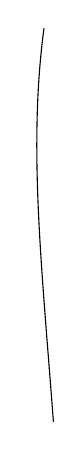
\begin{tikzpicture}\draw (0,0) .. controls (-.20,-1.5) and (-.03,-3) .. (.12,-5);\end{tikzpicture}}}}
\uline{Proposition} 11.$\overset{\handwritten{-}}{\underset{\handwritten{\vert}}{1}}1$. Soi\deleted{e}\handwritten{t}\deleted{nt $k$ un corps}, $G$ un \deleted{schéma en }groupe\deleted{s quasi-compact}\inserted{\handwritten{algébrique sur le}} \deleted{sur}\inserted{\handwritten{corps}} $k$. Les conditions suivantes sont équivalentes:

(i) $G$ est affine.

(ii) $G$ est quasi-affine.

(iii) On peut faire opérer $G$ fidèlement sur un\inserted{$k$-}schéma quasi-affine.

(iv) On peut faire opérer $G$ fidèlement sur un vec\deleted{o}\handwritten{t}oriel sur $k$ (\deleted{\illegible{1}}\handwritten{p}\deleted{\illegible{1}}\handwritten{a}s nécessairement de \deleted{t}\inserted{d}imension finie).

(v) \deleted{(\unsure{si|Si} $G$ est de type fini sur $k$),} $G$ est isomorphe à un sous-groupe fermé d'un groupe $\mathrm{Gl}(n)_k$ .

\uline{Démonstration}. On a (i)$\handwritten{\Rightarrow}$(ii) trivialement, et (ii)$\handwritten{\Rightarrow}$(iii), car $G$ opère fidèlement sur lui-même par translations à gauche. On a (iii)$\handwritten{\Rightarrow}$(iv) car si $G$ opère \deleted{fidèlement sur $X$ quasi-affine sur $k$, alors $G$ opère fidèle-\linebreak ment sur l'enveloppe affine $X'=\operatorname{Spec}(\handwritten{\unsure{\Gamma|I}}($}\inserted{sur $X$ quasi-compact et quasi-séparé sur $k$, il opère aussi} sur le vectoriel $\handwritten{\Gamma}(X,\underline{O}_X)$, grâce au fait que la formation de $f_{\handwritten{*}}(\underline{O}_X)$ ($f:X\handwritten{\to}\operatorname{Spec}k$ le morphisme structural) commute à tout changement de base $S\handwritten{\to}\operatorname{Spec}k$ (EGA IV 1.7.12); donc il opère sur l'enveloppe affine $X'=\operatorname{Spec}(\handwritten{\Gamma}(X,\underline{O}_X))$, et le morphisme canonique $X\handwritten{\to}X'$ est évidemment compatible avec l'action de $G$; ceci dit, si $X$ est quasi-affine i.e. $X\handwritten{\to}X'$ est une immersion ouverte, et si $G$ opère fidèlement sur $X$, il opère fidèlement sur $X'$, ou ce qui revient au même, sur le vectoriel $V=\handwritten{\Gamma}(X,\underline{O}_X)$, ce qui prouve l'implication (iii)$\handwritten{\Rightarrow}$(iv).

\deleted{S}\handwritten{\unsure{S|s}}upposons maintenant \deleted{d'abord $G$ de type fini, e}t\inserted{\handwritten{(iv), i.e.}} que $G$ opère fidèle-\linebreak ment sur le vectoriel $V$. Alors\handwritten{,}en vertu de 11.10\handwritten{,}$V$ est limite inductive de sous-es\deleted{ap}\handwritten{pa}ces vectoriels $V_i$ de di\deleted{em}\handwritten{me}nsion finie, stables sous l'action de $G$. Si $K_i$ est le noyau de l'action induite de $G$ sur $V_i$ , i.e. de $G\handwritten{\to}\underline{\operatorname{Aut}}_{\inserted{\handwritten{V_i}}}\deleted{\unsure{(V_i)}}$, alors $K_i$ est un sous-schéma fermé de $G$, et l'hypothèse que $G$ opère fidèlement s'exprime aussitôt par le fait que \deleted{$K_{\unsure{i|1|l}}=e$ (grou} l'intersection des $K_i$ est le sous-groupe unité de $G$. Comme $G$ est noethé-%
% archive sheet number: 48
